\chapter{Discussion}

\todo{
	**Things to avoid
	2Hyping findings-
	3Interpreting beyond what can be justified-
	4Extend in tangential topics-}

1-Intro - to be written when the section is more mature

2-What have we done:  a paragraph or two explaining the major findings and why are important.

\section{Validation of experimental results}
\subsection{Open loop simulation}
\todo{This was written in chapter 6.}
The main losses are the dissipation from the component in heat. Also the load is a power resistor and it changes the resistance if it is in operation. So we have not a constant load at the output as in the simulation. Another reason is the dead-time of the MOSFET and therefore the duty cycle is not exactly the same value as in the simulation. 

The table \ref{tab:ripple} compares the values of the ripples from the experiments with the values from the requirements in section \ref{sec:componentsizing} and the simulation results in appendix \ref{app:OL_ripple}. So in all three cases the measured ripples from the experiment are higher/lower than the values from the requirement. Here the reason.

\begin{table}[H]
	\centering
	\begin{tabular}{|>{\centering}p{3.5cm}|p{3cm}|p{3cm}|p{3cm}|}
		\hline
		\rowcolor{lightgray} \textbf{} & \textbf{Requirement} & \textbf{Simulation}  & \textbf{Experiment}   \tabularnewline \hline
		$\Delta V_{in}$ & 0.1\% & - & - \tabularnewline \hline
		$\Delta I_{L}$ & 10\% & 10\% & 9.86\% \tabularnewline \hline
		$\Delta V_{out}$  & 0.5\% & 0.5\% & 0.055\% \tabularnewline \hline
	\end{tabular}
	\caption{Voltage and current ripple.}
	\label{tab:ripple}
\end{table}

\todo{The output ripple was tested for buck mode instead of boost mode so mention here why. Stef}

\subsection{MPPT}


\section{Problems and limitations}
3-Explain main problems and limitations and how are handled. Be succinct, be frank but no apologetic. Explain implications of limitations.
\subsection{Layout improvement procedure and issues, title to be improved}
opto <--x-->driver voltage levels?

inductor saturation and so

pcb hot points

...
\subsection{output cap?}
\subsection{MPPT drifting and improvement and limitations of final control algorithm}
The development of an embedded control system requires the proper working of an algorithm. During the development process, the engineer might find that the code doesn't behave as intended. A common way of supporting the debugging process consists on the use of breakpoints, where the code is stopped and the variables' value might be read. However, as this feature is not supported by the used platform, and in the case of controlling physical systems its use would be limited to simulation, alternative techniques had to be used. The adopted approach consisted on outputting the FSMs state and relevant values for the current state at every code execution loop. The 'Timestamp' field is specially important during simulation in order to track specific events at determined times. See figure \ref{console_output}.

\begin{figure}[htbp]
	\begin{center}
		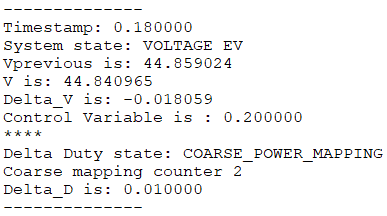
\includegraphics[width=0.5\textwidth]{../Pictures/P1/Discussion/console_output.png}
		\caption{Console output.}
		\label{console_output}
	\end{center}	
\end{figure}

In initial implementations of the control algorithm, the voltage evaluation was performed in the state next to the duty cycle change. After this change, the system experiences a transient stage where the input voltage and inductor current evolve into the new steady state value. If these variables are read during the transient, the control might infer that the PV panel is in a location of the P-V curve different than where it actually is. The MPPT becomes noisier under this scenario. In order to address this issue, an additional waiting state was added to the FSM governing the system. Another solution to the issue would be to decrease the MPPT algorithm periodicity. However this solution would lead to a decrease in system's responsiveness. However this drawback might be bearable by implementing a voltage controller aside from the MPPT.  

limitations of MPPT

\subsection{software filtering}
Although the voltage and current measurement is filtered, the signal read by the control system was noisy. This noise affected the MPPT algorithm disturbing its ability to reach the MPP. Such noise might have different sources within a lab with such a big amount of hardware equipment. There are many techniques in order to address noise issues, the used technique consists on the use of digital filtering (LPF). This digital filter is a  simple code that performs the filtering at a given frequency. Being a first order filter, it was simple and fast to implement and test. 
..
.

filtering image result
\subsection{Coil test}

\section{Future work}
This section will describe the planned future work of the project. This includes parts that were prioritized low or Simplified to achieve a working converter. Furthermore it includes improvements that was discovered during both the development and testing period of the project.

%4- Recommendations for future work. Make general statements. Items: a)what study is needed, b)Methods to be used, c)what is needed for that study.

\subsection{MPPT technique}
Even though the P\&O algorithm was implemented, initial research showed that the incremental conductance method could have been a better option.  Further research and simulations will have to be made for comparing the two methods. \todo{Write about what could be gained from changing MPPT, NHF.}

\subsection{V/I controller}


\subsection{Hardware improvements}
In the first iterations of the converter design, the driver circuits have been designed using isolated power supplies for the high side drivers. These are costly both in size and money wise. Because of that it's preferable to implement a bootstrap circuit for the drivers. An option for a driver including bootstrap could be UCC27211 \cite{boot_driver_datasheet}. This includes both a high and low side driver, such that only to IC's are necessary for the converter. The input threshold is below $2.8V$ for both sides, which means that a $5V$ optocoupler could be used for isolation. For cost and size optimization the optocouplers should be one quad optocoupler, instead of four singles. 
 
%bootstrap, change driver to the A version due to voltage levels and then change the optocouupler to a quad version, control system powered from pv-panel, \dots

\subsection{Coil design}
The coil used for the converter is reused from an earlier project. Measurements shows that it's oversized regarding current ratings. To achieve an optimal coil it should be designed for this specific converter. Both the core size and wire diameter depends on the wanted current rating of the converter \cite{underthehood}. Because of this it will be possible to lower both the cost and size of the coil. 

\subsection{Switching frequency limitations}

%\subsection{Component price, system size, optimization needed}
%Component prize and system size will be introduced during the other sections...

\subsection{Efficiency}
The main purpose of the MIC is to maximize the output efficiency of a PV-panel. To achieve that, the efficiency of the converter itself should be maximized. During the tests, the efficiency was measured to \textit{ADD SOME NICE DATA}\todo{Insert measured efficiency, NHF.}. Other papers shows that an efficiency of up to $95-96\%$ should be achievable\cite{underthehood}, \cite{efficient_buckboost}. 




